\documentclass[tikz,border=10pt]{standalone}
\usepackage{amsmath}
\usepackage{amssymb}
\usepackage{tikz}
\usetikzlibrary{arrows.meta,calc}

\definecolor{figazul}{RGB}{2,132,199}
\definecolor{figrojo}{RGB}{220,38,38}
\definecolor{figverde}{RGB}{22,163,74}

\begin{document}
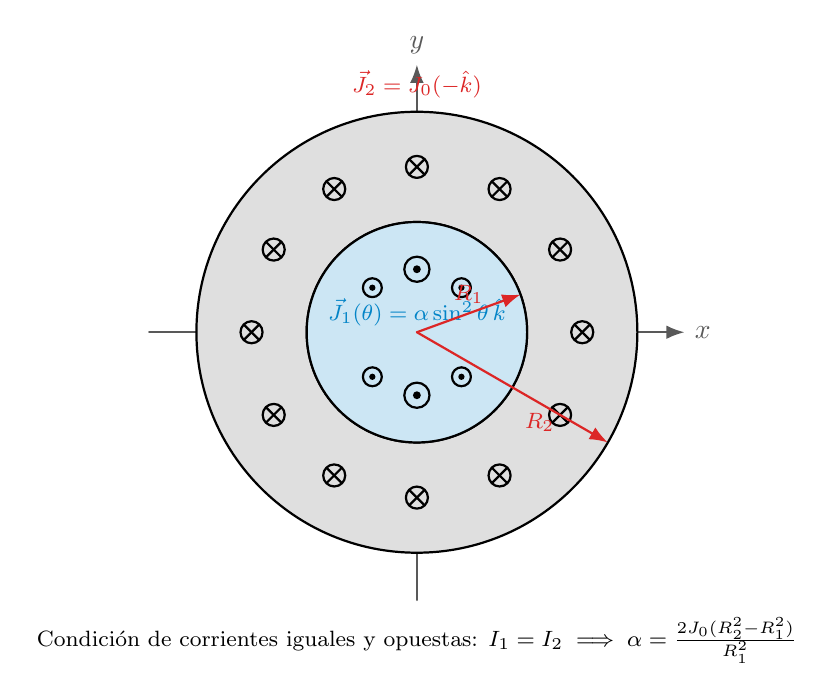
\begin{tikzpicture}[>=Latex, line cap=round, line join=round]
  % Ejes cartesianos
  \draw[->, thick, color=gray!70!black] (-3.4,0) -- (3.4,0) node[right] {$x$};
  \draw[->, thick, color=gray!70!black] (0,-3.4) -- (0,3.4) node[above] {$y$};

  % Cascarón exterior: R1 = 1.4, R2 = 2.8
  \draw[thick, fill=gray!25] (0,0) circle (2.8);
  \draw[thick, fill=white] (0,0) circle (1.4);

  % Cilindro interior: radio R1 = 1.4
  \draw[thick, fill=figazul!20] (0,0) circle (1.4);

  % Distribución angular en el interior: J1(theta) = alpha * sin^2(theta)
  % Cero en theta = 0, 180 (eje x), máximo en theta = 90, 270 (eje y)
  % Símbolos de corriente saliente (odot) proporcionales en el interior
  % En eje y: máximo
  \draw[thick] (0, 0.8) circle (0.16); \fill (0, 0.8) circle (0.05);
  \draw[thick] (0, -0.8) circle (0.16); \fill (0, -0.8) circle (0.05);
  % En 45, 135, 225, 315: intermedio
  \foreach \ang in {45, 135, 225, 315} {
    \draw[thick] (\ang:0.8) circle (0.12); \fill (\ang:0.8) circle (0.04);
  }
  \node[font=\footnotesize, color=figazul] at (0, 0.25) {$\vec{J}_1(\theta) = \alpha\sin^2\theta\,\hat{k}$};

  % Cascarón exterior: J2 = J0 (-k, entra: otimes) uniforme
  \foreach \ang in {0, 30, 60, 90, 120, 150, 180, 210, 240, 270, 300, 330} {
    \draw[thick] (\ang:2.1) circle (0.14);
    \draw[thick] (\ang:2.1) ++(-0.09,-0.09) -- ++(0.18,0.18);
    \draw[thick] (\ang:2.1) ++(-0.09,0.09) -- ++(0.18,-0.18);
  }
  \node[above, font=\footnotesize, color=figrojo] at (0, 2.85) {$\vec{J}_2 = J_0(-\hat{k})$};

  % Radios y cotas con flechas
  \draw[->, thick, color=figrojo] (0,0) -- (20:1.4);
  \node[above, color=figrojo, font=\footnotesize] at (20:0.7) {$R_1$};

  \draw[->, thick, color=figrojo] (0,0) -- (-30:2.8);
  \node[below, color=figrojo, font=\footnotesize] at (-30:1.8) {$R_2$};

  % Leyenda
  \node[below, font=\footnotesize] at (0, -3.5)
    {Condición de corrientes iguales y opuestas: $I_1 = I_2 \implies \alpha = \frac{2J_0(R_2^2 - R_1^2)}{R_1^2}$};
\end{tikzpicture}
\end{document}
